\documentclass[11pt]{beamer}

\usepackage{amsmath, graphicx, natbib, verbatim, color}
\usepackage{colortbl}
%\usetheme{CambridgeUS}

\useoutertheme{infolines}
\usetheme{default}

\setbeamertemplate{navigation symbols}{}
\setbeamertemplate{headline}{}


\setbeamertemplate{navigation symbols}{}



\definecolor{forest}{rgb}{.15, .5, .15}
\definecolor{brick}{rgb}{.7, .15, .15}
\definecolor{darkgreen}{rgb}{.15, .5, .15}
\definecolor{darkred}{rgb}{.7, .15, .15}
\definecolor{darkblue}{rgb}{.15, .15, .7}
\definecolor{Green}{rgb}{0.2,1,0.2}

\usepackage[english]{babel}
\usepackage[latin1]{inputenc}
\usepackage{times}
\usepackage[T1]{fontenc}

\setlength{\itemsep}{15em}

\title[Predicting survival]% (optional, with long titles)
{Robust Survival Prediction via Linear Transformation Models} 
\author[Betts, Harrington]{Keith Betts \\
Dave Harrington \\
 \texttt{dph@jimmy.harvard.edu} }

\institute % (optional)
[AG, Harvard] {{\color{brick} Analysis Group, Harvard University}}

\date{7 August 2014}

\begin{document}


\begin{frame}

\titlepage

\end{frame}

%%%%%%

\begin{frame}{Graphic from 1993 \textsl{NEJM} paper, prognosis in
non-Hodgkin's lymphoma}


\begin{columns}[c]

\begin{column}{0.65\textwidth}


\begin{center}
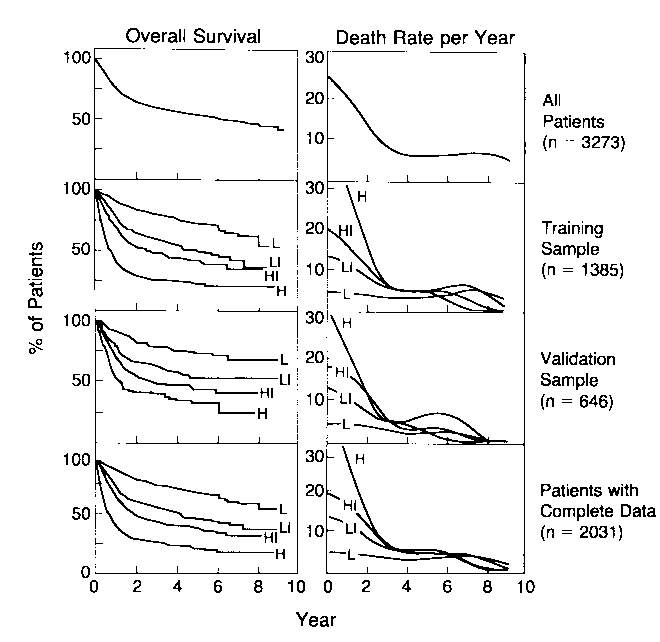
\includegraphics[width=1.0\textwidth]{./figures/nejm_curves.pdf}
\end{center}

\end{column}


\begin{column}{0.35\textwidth}

Covariates in model: 
\begin{itemize}

  \item Age

  \item Stage

  \item Tumor size

  \item Extent of disease

  \item Performance status

\end{itemize}
\end{column}


\end{columns}

\end{frame}


\begin{frame}{`Prognostic models' now widely used}

Models that predict the risk of disease or disease progression
have a long history in medical literature.

\begin{itemize}
  \item Gail model for breast cancer risk (\textsl{JNCI}, 1989)

  \item N. Cook's work in cardiovascular disease (\textsl{JAMA, NEJM})

  \item Mayo Clinic model in primary biliary cirrhosis (\textsl{Hep}, 1989)

  \item Models for Cardiovascular disease from Framingham Heart
  Study (D'Agostino, \textsl{Circ}, 1998, 2004, 2008)

  \item Coronary Heart Disease Policy Model, (Weinstein et. al,
  \textsl{Am J Pub Health}, 1987)

  \item Non-Hodgkin's lymphoma, (Shipp, et al. \textsl{NEJM}, 1993)


\end{itemize}

\end{frame}

\begin{comment}
\begin{frame}{Simple taxonomy of analysis goals}

\begin{itemize}
  
  \item Predict event times (generally difficult), or at least interval
  containing event time, estimate misclassification rate

  \item Estimate risk strata, with misclassification rates
 
  \item \textcolor{forest}{Predict occurrence of an event beyond a
  given time, estimate error}


  \item \textcolor{forest}{Estimate incremental value of nested
  models.}

  \begin{itemize}
 
  \normalsize
    \item Especially important in era of biomarkers,
    genomic/genetic signatures. 
  
  \end{itemize}

\end{itemize}

\end{frame}

\end{comment}

\begin{frame}{Sample of important methodologic literature,
prediction with event time data}

  \begin{itemize}

  \item Measures of explained variation with event time data, Korn
  and Simon, 1990, 
  
  \item Prediction error, Graf et. al, 1999
  
  \item Haegerty, et al., 2000 
  
  \item Gerds and Schumacher, 2006 

  \item Cai, Tian, Solomon, Uno, Wei (2007a, 2007b, 2008)

  \end{itemize}

\end{frame}


\begin{frame}{Our general approach}

\begin{itemize}

\item Use flexible class of linear transformation models for
censored data

  \item Evaluate time-dependent mean-squared error of prediction,
  and its standard error
  
  \item Avoid bias in apparent error rate

  \item Obtain unbiased estimates of error rates when model is
  misspecified

 \end{itemize}

\end{frame}

\begin{frame}{Notation and Models}

\begin{itemize}
  \item $T = $ event time, $C = $ potential censoring time, $Z = $
  $p$-dimensional vector of covariates

  \item Observed time $\tilde{T} = \min(T,C)$, $\delta = (T \leq C)$

  \item $S(t|Z) = \Pr(T>t | Z)$

  
   \item Semi-parametric Linear Transformation Model

      \begin{equation*}
        \textcolor{darkblue}{h(T)} = - \beta^T Z +
        \textcolor{forest}{\epsilon},
     \end{equation*}
\vspace{-.5em}

   $\textcolor{darkblue}{h(\cdotp)}$ is a unknown monotone strictly
   increasing function, \textcolor{forest}{$\epsilon$} has `known'
   distribution.

  \item Equivalent to 

   \begin{equation*}
   g^{-1}(S(t|Z)) = h(t) + \beta^T Z,
   \end{equation*}
with  $g^{-1} = 1 - F_\epsilon $

\end{itemize}


\end{frame}

\begin{frame}{Goal}

\begin{itemize}

\item Predict survival probability, 

  \begin{equation*}
  \hat{S}(t | Z^0) = g(\hat{h}(t,\hat{\beta}) 
     + \hat{\beta}^T Z^0)
  \end{equation*} 
  
  for an `out of sample' individual.

\item Estimate mean squared error of prediction (MSEP) as a
function of time, 
\begin{equation*}
\overline{\text{MSEP}}(t, \hat{S}, G) = E_{T, Z} \{I(T > t) - 
\hat{S}(t|Z) \}^2,
\end{equation*}
even when working model is wrong.

\item  This is expected Brier score, originally used in weather
prediction

\end{itemize}

\end{frame}


\begin{frame}{Assumptions}

\begin{itemize}
  
  \item  $(T \perp C) | Z$

  \item $Z$ is bounded

  \item $G(t | Z) = \Pr (C > t | Z)$ can be consistently estimated

  \item An assortment of regularity conditions

\end{itemize}

\vspace{0.20in}
Formulation for \textsl{MSEP} similar to Graf, Gerds.

\vspace{0.20in}

Proofs rely on work by H. Uno, T Cai, L Tian and LJ Wei on
asymptotics of mis-specified models

\end{frame}


\begin{frame}{Estimating equations and main results}

\begin{itemize}
\vspace{.5em}
\item \textcolor{brick}{Estimating Equations}

\begin{small}
\begin{eqnarray*}
  \textcolor{forest}{U_1(h(t), \beta)} &=& \sum_{i=1}^n 
     \left[I(\tilde{T}_i \geq t) - g(h(t) + \beta^T Z_i)
   \hat{G}(t | Z)\right]  \\
   \textcolor{darkblue}{U_2(\hat{h}(t, \beta), \beta)} 
      &=& \sum_{i=1}^n \int_{\tau_a}^{\tau_b}
      Z_i \left[ I (\tilde{T}_i \geq t) - g(\hat{h}(t, \beta) + \beta^T Z_i)
      \hat{G}(t | Z)\right] dt 
\end{eqnarray*}
\end{small}
  \item \textcolor{brick}{Main results:}  Even when $S$ is
  mis-specified
\begin{itemize}

\normalsize

\item Unique solutions $\hat{h}(t, \beta)$ and $h_*(t, \beta)$ for
$U_1(h(t), \beta)$ and its expectation for a fixed $\beta$

\item Unique solutions $\hat{\beta}$ and $\beta_*$, for $U_2(\hat{h}(t),
\beta)$ and $E[U_2(h_*(t), \beta)]$

\item Consistency, $\hat{\beta} \xrightarrow{p} \beta_*$

\item Uniform consistency, $\text{sup}_t | 
\hat{h}(t, \hat{\beta}) - h_*(t, \beta_*) |
\xrightarrow{p} 0$


\end{itemize}

\end{itemize}

\end{frame}


\begin{frame}{Results \ldots}


 There exists a survivor function $\bar{S}$ such that
 
 \begin{itemize}

 \item  $\sqrt{n} \{ \hat{S}(t | Z^0) - \bar{S}(t | Z^0) \}$
 converges to a Gaussian process, and

\begin{equation*}
\overline{\text{MSEP}}(t, \bar{S}, G) = 
\textcolor{forest}{E_{Z} \{S(t | Z) - \bar{S}(t|Z) \}^2} + 
\textcolor{darkblue}{E_Z \{ S(t|Z) (1 - S(t|Z) \}}
\end{equation*}

 \item Limiting distribution has complicated covariance structure but
 does  not  depend on censoring distribution, even when $S$
 has been mis-specified.

\end{itemize}
\end{frame}

\begin{frame}{Estimation of \textsl{MSEP}}

\begin{itemize}

\item \textsl{MSEP} estimate
\begin{equation*}
\widehat{\text{MSEP}}(t, \hat{S}, \hat{G}) = n^{-1}
\sum_{i=1}^n \textcolor{forest}{\{ I(\tilde{T}_i \geq t) - 
\hat{S}(t | Z_i) \}^2} \textcolor{darkblue}{w(t, \hat{G}, Z_i)},
\end{equation*}
where
\[
\textcolor{darkblue}{w(t, \hat{G}, Z_i) = \frac{I(\tilde{T}_i \leq t) 
\delta_i}{\hat{G}(\tilde{T}_i-|Z_i)} + 
\frac{I(\tilde{T}_i > t)}{\hat{G}(t|Z_i)}}.
\]

\item Uniform consistency
\begin{equation*}
\text{sup}_t | \widehat{\text{MSEP}}(t, \hat{S}, \hat{G}) 
     - \overline{\text{MSEP}}(t, \bar{S}, G) | \xrightarrow{p} 0.
\end{equation*}

\item Inference on $\sqrt{n} \{\widehat{\text{MSEP}}(t, \hat{S}, \hat{G}) -
\overline{\text{MSEP}}(t, \bar{S}, G) \}$ using perturbation resampling.

\end{itemize}
\end{frame}


\begin{frame}{Cross validation to estimate \textsl{MSEP}}

\begin{itemize}

\item Ideally: Independent training and test datasets

\item Apparent error will be overly optimistic

\item K-fold cross validation
\begin{equation*}
\widehat{\text{MSEP}}^{\text{CV}} = \frac{1}{K} 
\sum_{k=1}^K \widehat{\text{MSEP}}(\hat{h}^{(-k)}
(t, \hat{\beta}^{(-k)}), \hat{\beta}^{(-k)}),
\end{equation*}
where $\hat{h}^{(-k)}(t, \hat{\beta}^{(-k)})$, 
and $\hat{\beta}^{(-k)}$ are estimated using the data in the $K-1$
datasets not including set $k$.

 \item Simulations show procedure works reasonably well -- more
 interesting to look at examples.

\end{itemize}
\end{frame}


\begin{frame}{Lymphoma Data}

\begin{columns}[c]

\begin{column}{0.65\textwidth}


\begin{center}
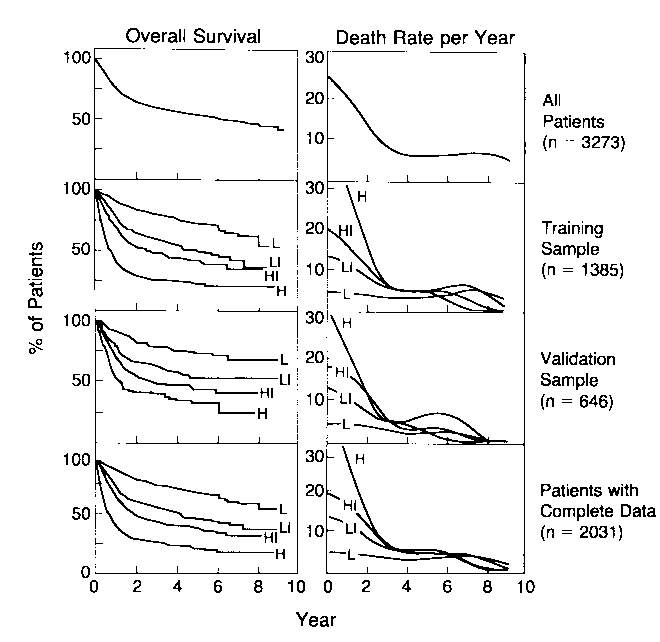
\includegraphics[width=1.0\textwidth]{./figures/nejm_curves.pdf}
\end{center}

\end{column}


\begin{column}{0.35\textwidth}

Covariates in model: 
\begin{itemize}

  \item Age

  \item Stage

  \item Tumor size

  \item Extent of disease

  \item Performance status

\end{itemize}
\end{column}


\end{columns}

\end{frame}

\begin{comment}

\begin{frame}{Lymphoma data: \textsl{MSEP}, risk
categories as categorical covariate}

\begin{center}
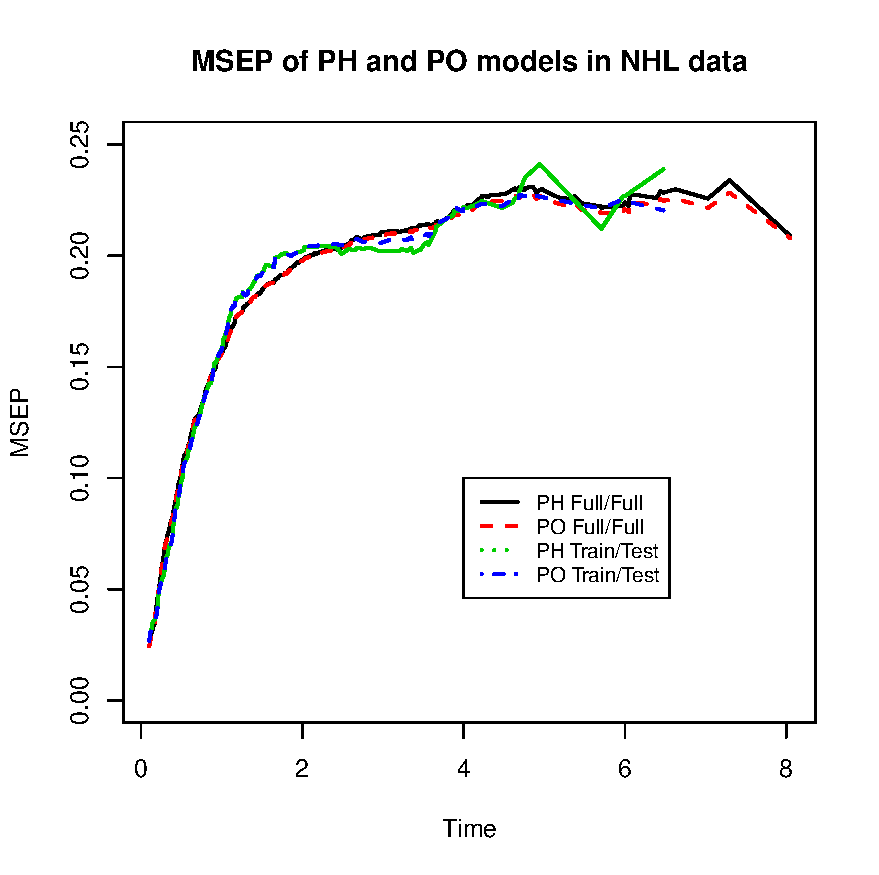
\includegraphics[width=0.65\textwidth]{./figures/4riskgroups.pdf}
\end{center}
\end{frame}

\end{comment}

\begin{frame}{Lymphoma data: \textsl{MSEP}, original binary
covariates}

\begin{center}
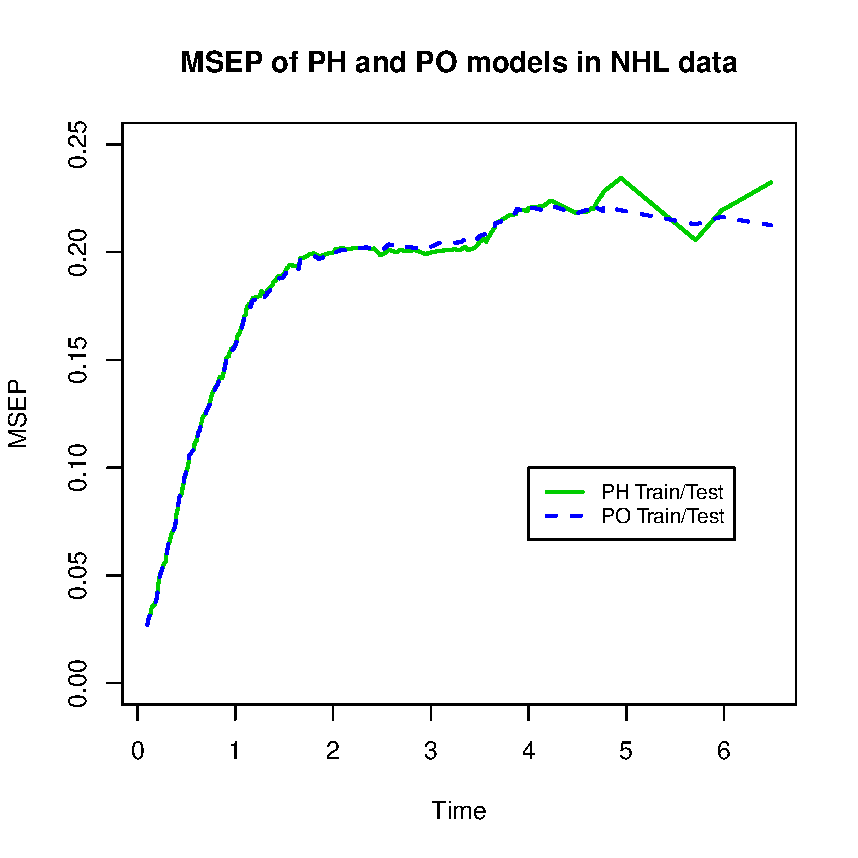
\includegraphics[width=0.7\textwidth]{./figures/NHLtraintest.pdf}
\end{center}
\end{frame}


\begin{frame}{Lymphoma data: mean squared error of prediction with
confidence intervals, validation dataset}

\begin{center}
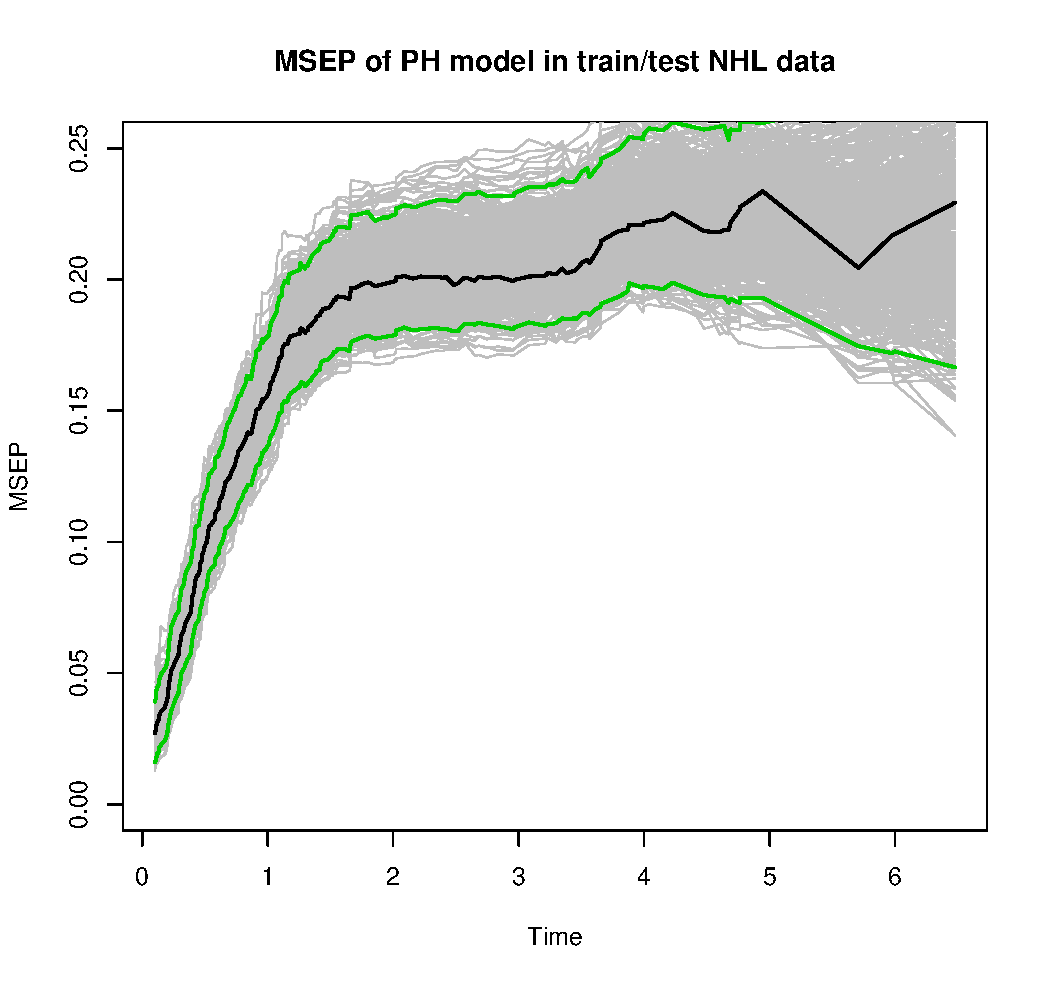
\includegraphics[width=0.7\textwidth]{./figures/NHLMSEPvalidationCI.pdf}
\end{center}

\end{frame}

\begin{frame}{Multiple Myeloma}

Myeloma study from Eastern Cooperative Oncology Group (E9486)

%%%% fix this slide

\begin{itemize}

\item Randomized trial of three treatments in multiple myeloma, no
survival differences observed among 653 patients

\vspace{.5em}

\item 295 participant specimens randomly chosen for analysis of a deletion
on long arm of chromosome 13 (13q-). 270 deaths


   \item Originally reported in {\sl JCO} (1999), {\sl Blood} (2001),
    {\sl Biometrics} (2002)

\end{itemize}

\end{frame}

\begin{frame}{Myeloma: Value of an additional marker?}
%\vspace{.25in}
\begin{center}
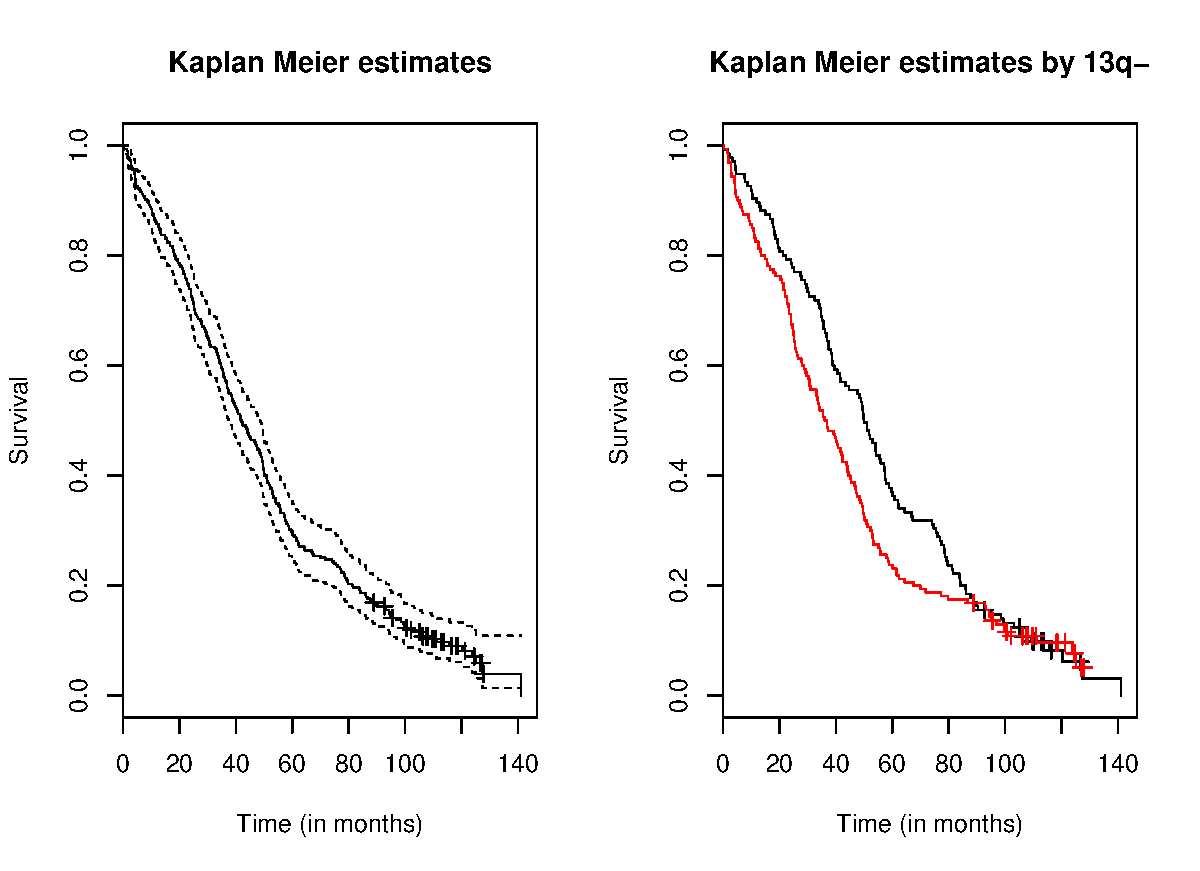
\includegraphics[scale=.53]{./figures/myeloma_km.pdf}
\end{center}
\end{frame}

\begin{comment}

\begin{frame}{Simple PH model with, without $13q-$ biomarker}
\begin{footnotesize}
\begin{table}[ht]
\begin{center}
\begin{tabular}{rrr}
  \hline
  & Without $ 13q-$ & With $13q-$ \\
  & Coeff. (std. err.) & Coeff. (std. err.) \\
  \hline
$\Delta 13$ & - & -0.68 (.21)\\ 
 $\beta_2$ micro & -0.55 (.26) & -0.53 (.25)\\ 
 Creatine & -0.76 (.27)& -0.88 (.28)\\ 
  IL-6 & -0.51 (.20)& -0.52 (.20)\\ 
  C-reactive & -0.91 (.22)& -0.89 (.23)\\ 
   \hline
\end{tabular}
\end{center}
\end{table}
\end{footnotesize}
\end{frame}

\end{comment}

\begin{frame}{Working PH model coefficient estimates}
\begin{footnotesize}
\begin{table}[ht]
\begin{center}
\begin{tabular}{rrrrr}
  \hline
 & Base & Base $+ \Delta 13$ & Stepwise & Stepwise $+ \Delta 13$ \\ 
  \hline
$\Delta 13$ & - & -0.57   (.21)& - & -0.68 (.21)\\ 
 Albumin  & 0.30 (.27)& 0.25   (.27)& - & - \\ 
 $\beta_2$ micro & -0.48 (.25)  & -0.48 (.26)& -0.55 (.26) & -0.53 (.25)\\ 
 Creatine & -0.65 (.28)  & -0.80 (.29)& -0.76 (.27)& -0.88 (.28)\\ 
 Hemoglobin& -0.31 (.30)  & -0.29 (.31)& - & - \\ 
 IgA & 0.10 (.22) & 0.10   (.24)& - & - \\ 
 IgG & -0.42 (.32)& -0.46   (.32)& - & - \\ 
 Light chain ($\kappa$) & -0.67  (.39) & -0.76 (.38)& - & - \\ 
 \% plasma cells  & -0.78 (.23)  & -0.69 (.24)& - & - \\ 
 PCLI & 0.49 (.24)  & 0.41 (.23)& - & - \\ 
  IL-6 & -0.42 (.21) & -0.44 (.21)& -0.51 (.20)& -0.52 (.20)\\ 
  C-reactive & -0.88 (.23)& -0.87 (.25)& -0.91 (.22)& -0.89 (.23)\\ 
  Durie-Salmon & -0.07 (.25)& -0.16 (.25)& - & - \\ 
   \hline
\end{tabular}
\end{center}
\end{table}
\end{footnotesize}
\end{frame}



\begin{frame}{MSEP for Myeloma models}
\vspace{-0.25in}
\begin{center}
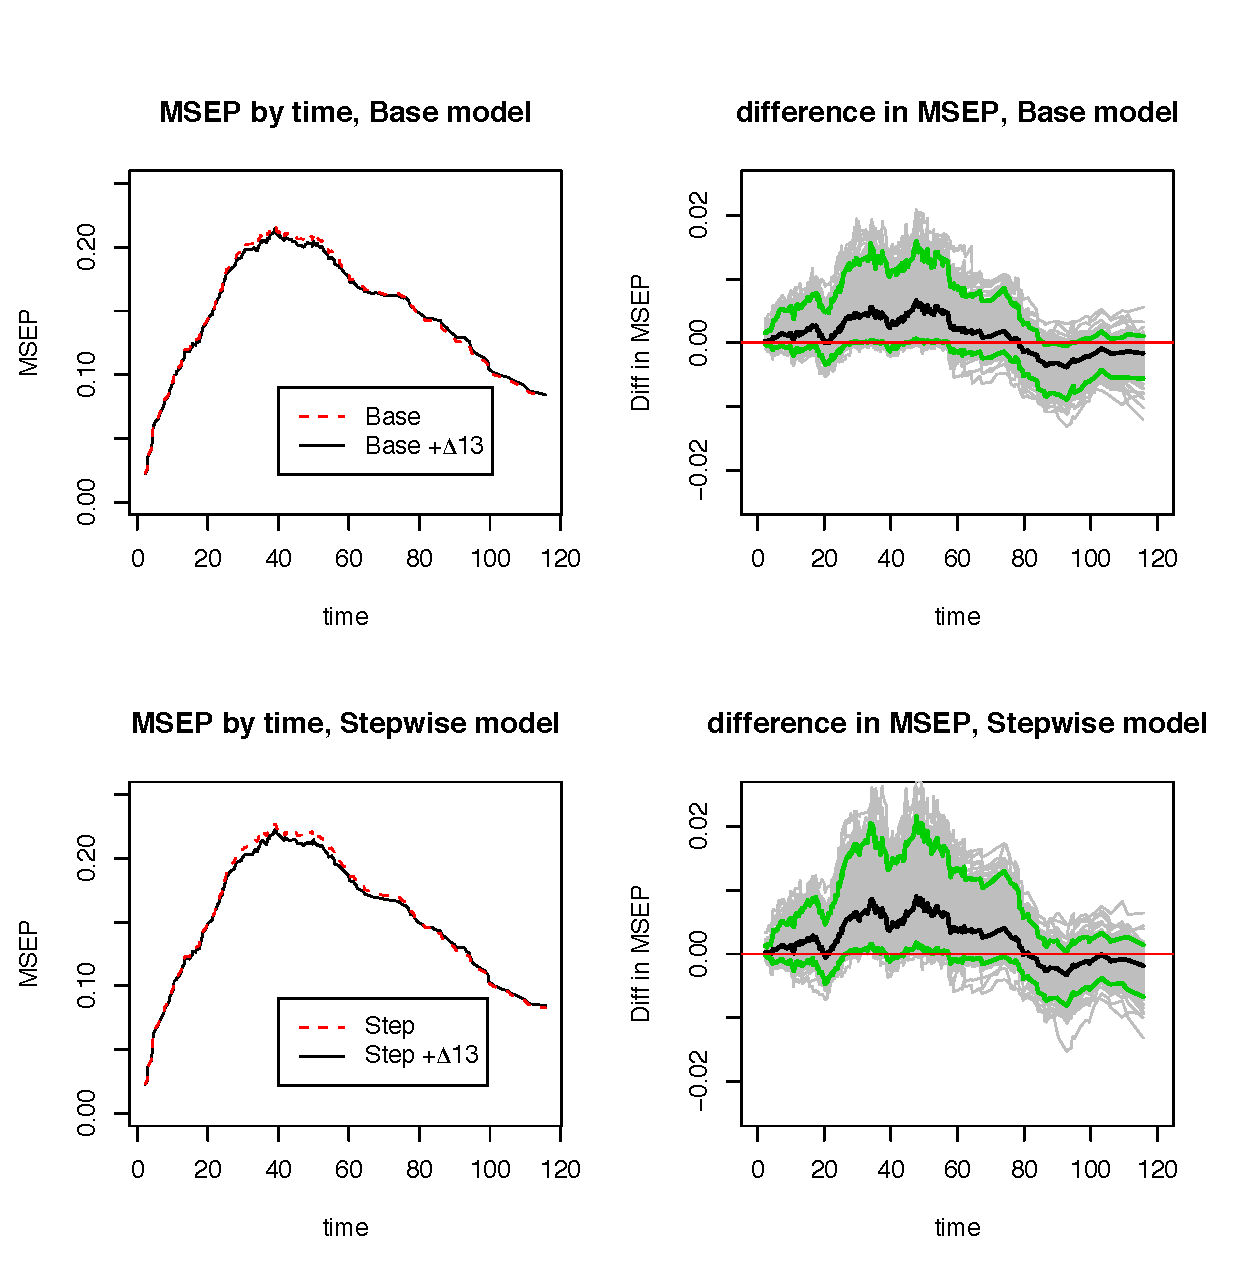
\includegraphics[scale=0.40]{./figures/myeloma_msep_full.pdf}
\end{center}
\end{frame}

\begin{frame}{Some simulations}


{True vs. apparent vs. cross-validated \textsl{MSEP} for the Linear
Transformation Model (LTM) and the Cox model evaluated at $1^{st}$
quartile and median for simulated data.}


\begin{small}
\begin{center}
\begin{tabular}{rrrrrrrrr}
  \hline
   & & & $q={.25}$  & & & & $q={.5}$ & \\ \cline{3-5} \cline{7- 9} 
 & & Truth & App. & CV &   &Truth & App. &CV  \\   \hline
A & $\text{MSEP}_{\text{LTM}}$ &  .131 & .134& .132  &   & .132 & .134 & .130  \\
      & $\text{MSEP}_{\text{Cox}}$ &     - & .133 & .131 &   & - & .134 & .131  \\
\textcolor{brick}{B} & $\text{MSEP}_{\text{LTM}}$ & \textcolor{brick}{
.161} & .169& .165  &   & \textcolor{brick}{.210} & .215 & .211  \\
      & $\text{MSEP}_{\text{Cox}}$ &     - & .168 & .164 &   & - & .214 & .211  \\
C & $\text{MSEP}_{\text{LTM}}$ &  .136 & .142& .139  &   & .145 & .152 & .147   \\
      & $\text{MSEP}_{\text{Cox}}$ &     - & .155 & .152 &   & - & .159 & .154  \\
\hline
\end{tabular}
\end{center}
 
 \hspace{1in} \textsl{A:}  PH data, correctly fit with LTM\\
  \hspace{1in} \textsl{\textcolor{brick}{B:}}  PH data, correct LTM, but neglected covariate \\
  \hspace{1in} \textsl{C:}  PH data, PO model fit for LTM

\end{small}

%\end{table}


\end{frame}


\begin{frame}{Limitations}

\begin{itemize}
  \item Estimating equations are not efficient

  \item Must estimate censoring distribution (correctly!)

  \item \textsl{MSEP} not easily interpreted

  \item Falls short of predicting event times

\end{itemize}

\end{frame}



\end{document} 
